\documentclass{beamer}
\usepackage{tikz} %for mindmap
\usetikzlibrary{mindmap} %for mindmap
\usepackage{pgfpages}
\usepackage[backend=bibtex]{biblatex}
\usepackage{multicol}
\usepackage{textpos}
\setbeameroption{hide notes} % Only slides
%\setbeameroption{show only notes} % Only notes
%\setbeameroption{show notes on second screen=right} % Both
\bibliography{../../papers/references.bib}
\setbeamerfont{footnote}{size=\small}
%\AtEveryCitekey{\clearfield{title}}

%
% Choose how your presentation looks.
%
% For more themes, color themes and font themes, see:
% http://deic.uab.es/~iblanes/beamer_gallery/index_by_theme.html
%
\mode<presentation>
{
  \usetheme{Warsaw}      % or try Darmstadt, Madrid, Warsaw, ...
  \usecolortheme{default} % or try albatross, beaver, crane, ...
  \usefonttheme{default}  % or try serif, structurebold, ...
  \setbeamertemplate{navigation symbols}{}
  \setbeamertemplate{caption}[numbered]
} 

\usepackage[english]{babel}
%\usepackage[utf8x]{inputenc} %Doesn't play well with biblatex
\usepackage{amssymb}
\usepackage{bm}
\usepackage{color}
\usepackage{graphicx}

\newcommand{\red}[1]{{\color{red}{#1}}}
\newcommand{\ket}[1]{\left| #1 \right>}
\newcommand{\bra}[1]{\left< #1 \right|}
\newcommand{\braket}[2]{\left< #1 | #2 \right>}
\newcommand{\ketbra}[2]{\left| #1 \right> \left< #2 \right|}
\newcommand{\expect}[1]{\left< #1 \right>}
\newcommand{\fpij}{f_p(r_{ij})}
\newcommand{\vpij}{v_p(r_{ij})}
\newcommand{\Opij}{\mathcal{O}_{ij}^p}
\newcommand{\fOpij}{\sum\limits_{i<j}\sum\limits_p \fpij\Opij}
\newcommand{\fqkl}{f_q(r_{kl})}
\newcommand{\Oqkl}{\mathcal{O}_{kl}^q}
\newcommand{\fOqkl}{\sum\limits_{k<l}\sum\limits_q \fqkl\Oqkl}
\newcommand{\fOqklip}{\sum\limits_{k<l,\mathrm{ip}}\sum\limits_q \fqkl\Oqkl}
\newcommand{\fOqklquad}{\sum_{\substack{k<l\\ij \ne kl}}\sum\limits_q \fqkl\Oqkl}
\newcommand{\f}[2]{f_{#1}(r_{#2})}
\renewcommand{\O}[2]{\mathcal{O}_{#2}^{#1}}
\newcommand{\fO}[2]{\sum\limits_{#1} f_{#1}(r_{#2})\mathcal{O}_{#2}^{#1}}
\newcommand{\R}{\mathbf{R}}
\newcommand{\dt}{\Delta\tau}
\newcommand{\ti}{\bm{\tau}_i}
\newcommand{\tj}{\bm{\tau}_j}
\newcommand{\si}{\bm{\sigma}_i}
\newcommand{\sj}{\bm{\sigma}_j}
\newcommand{\sfont}{6}
\newcommand{\sspace}{10.2}
\newcommand{\Oijp}{\mathcal{O}^p_{ij}}

\title[Improved Trial Wave Functions for Nuclear QMC]{Improved Trial Wave Functions for Nuclear Quantum Monte Carlo}
\author[Cody L. Petrie, cody.petrie@asu.edu]{Cody L. Petrie\\
Advisor: Kevin Schmidt\\~\\
INT Program INT-18-2b Advances in Monte Carlo Techniques for Many-Body Quantum Systems \\
July 30 - September 7, 2018}
\institute{Arizona State University \\ Tempe, AZ}
\date{}

\begin{document}

\begin{frame}
  \titlepage
\end{frame}

\iffalse
\begin{frame}{Mind Map Outline}
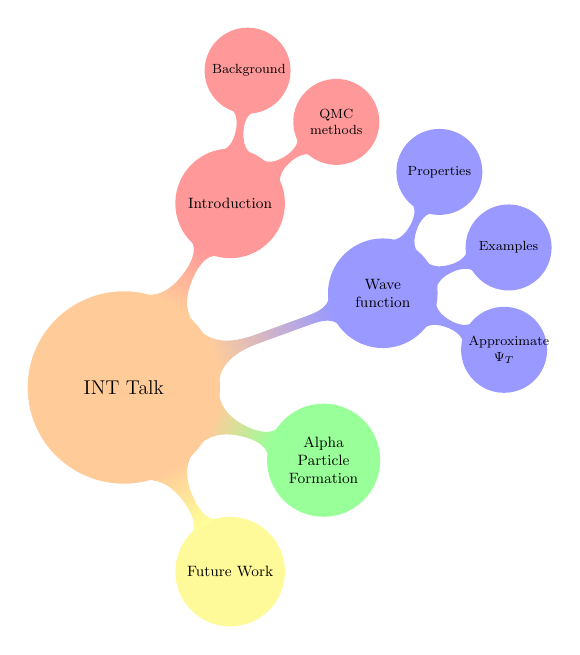
\begin{tikzpicture}[mindmap, grow cyclic, every node/.style=concept, concept color=orange!40]
\tikzset{level 1 concept/.append style={sibling angle=-40,level distance = 27mm}}
\tikzset{level 2 concept/.append style={sibling angle=-45,level distance = 17mm}}
\tikzset{level 3 concept/.append style={sibling angle=-45,level distance = 12mm}}
\tikzset{level 4 concept/.append style={sibling angle=-45,level distance = 10mm}}
\tikzset{every node/.append style={scale=0.6}}

\node[scale=1.0]{INT Talk}
   child[concept color=red!40]{node{Introduction}
      child{node{Background}}
      child{node{QMC methods}}
   }
   child[concept color=blue!40, level distance=35mm]{node{Wave function}
      child{node{Properties}}
      child{node{Examples}}
      child{node{Approximate $\Psi_T$}}
   }
   child[concept color=green!40]{node{Alpha Particle Formation}}
   child[concept color=yellow!40]{node{Future Work}}
;

\end{tikzpicture}
\end{frame}

% Commands to include a figure:
%\begin{figure}
%\includegraphics[width=\textwidth]{your-figure's-file-name}
%\caption{\label{fig:your-figure}Caption goes here.}
%\end{figure}

%\fontsize{\sfont}{\sspace}\selectfont
\begin{frame}{Outline}

{\tiny Story: QMC has been an effective way to do nuclear physics. What is QMC. There are other ways to improve QMC (like better potentials, 3N forces, etc.) but I am going to focus on the trial wave function. Why is the trial wave function so important. What have they done in the past (what improvements did they see)? So what did you do (are you doing). What improvements did you see? What do you plan on using them for in the future? What other improvements will you use in the future?
\begin{itemize}
   \item History of QMC including some results. Maybe include some of the weaknesses.
   \item What is QMC?
   \begin{itemize}\fontsize{\sfont}{\sspace}\selectfont
      \item VMC
      \item DMC/AFDMC
   \end{itemize}
   \item Trial wave function and why it's so important
   \begin{itemize}\fontsize{\sfont}{\sspace}\selectfont
      \item Slater Dets (and Pfaffians)
      \item Jastrow and linear correlations
      \item Quadratic correlations
      \begin{itemize}\fontsize{\sfont}{\sspace}\selectfont
         \item Results
      \end{itemize}
   \end{itemize}
   \item Other correlations
   \begin{itemize}\fontsize{\sfont}{\sspace}\selectfont
      \item Exponential correlations
      \item Ale's correlations and $T^2$ fix
   \end{itemize}
   \item Application to $\alpha$-clustering
   \begin{itemize}\fontsize{\sfont}{\sspace}\selectfont
      \item Stefano's original results
      \item Results with quadratic correlations
   \end{itemize}
\end{itemize}}
\end{frame}

\begin{frame}{Nuclear Many Body Problem}
   \begin{equation*}
      \left<H\right> = \bra{\Psi}H\ket{\Psi} = \int\Psi^*(\bm{R})H\Psi(\bm{R}) d\bm{R}
   \end{equation*}
   \begin{equation*}
      H = \sum\limits_{i=1}^A \frac{\bm{p}^2}{2m} + \sum\limits_{i<j} v_{ij} + \sum\limits_{i<j<k} V_{ijk} + \ldots
   \end{equation*}
   \begin{itemize}
      \item There are a number of ways to solve this problem.
      \begin{itemize}
         \item QCD
         \begin{itemize}
            \item Lattice QCD
         \end{itemize}
         \item No-core shell model
         \item Coupled-cluster
         \item Self consistent Green's function method
         \item Quantum Monte Carlo
      \end{itemize}
   \end{itemize}
   \red{Should I have a slide for each method or should I have some popup information about each and just describe them here?}
   \\\red{Can they be clumped into different styles and talked about together on slides?}
\end{frame}

% Uncomment these lines for an automatically generated outline.
\begin{frame}{Outline}
  \tableofcontents
\end{frame}
\fi

\begin{frame}{Outline}
\begin{itemize}
   \item Quantum Monte Carlo Methods
   \begin{itemize}
      \item VMC
      \item DMC
      \item AFDMC
   \end{itemize}
   \item Trial Wave Functions
   \begin{itemize}
      \item Properties
      \item Quadratic Correlations
      \item Exponential Correlations
   \end{itemize}
   \item Application
\end{itemize}
\end{frame}

\section{QMC Methods}
\subsection{VMC}
\begin{frame}{Variational Monte Carlo}
\begin{itemize}
   \item Variational principle:
   \begin{equation*}
      \left<H\right> = \frac{\bra{\Psi_T}H\ket{\Psi_T}}{\braket{\Psi_T}{\Psi_T}} \ge E_0
   \end{equation*}
   \item The variational energy is then
   \begin{equation*}
      E_V = \frac{\int\psi_T^*(\R)H\psi_T(\R)d\R}{\int\psi_T^*(\R)\psi_T(\R)d\R} \ge E_0
   \end{equation*}
   \item To use Monte Carlo integration this is written as
   \begin{equation*}
      E_V = \int P(\R)E_L(\R) d\R \approx \frac{1}{N}\sum\limits_{n=1}^N E_L(\R_n)
   \end{equation*}
\end{itemize}
\end{frame}

\begin{frame}{Variational Monte Carlo}
\begin{itemize}
   \item We can do that if we multiply by $\Psi_T(\R)\Psi_T^{-1}(\R)$.
   \begin{align*}
      P(\R) &= \frac{|\Psi_T(\R)|^2}{\int|\Psi_T(\R)|^2d\R} \\
%      E_L(\R) &= \Psi_T^{-1}(\R) H \Psi_T(\R)
      E_L(\R) &= \frac{\Psi_T^*(\R) H \Psi_T(\R)}{\Psi_T^*(\R) \Psi_T(\R)}
   \end{align*}
   \item Monte Carlo integration gives
   \begin{equation*}
      E_V \approx \frac{1}{N} \sum\limits_{n=1}^N E_L(\mathbf{R_n}),
   \end{equation*}
   where the $\R_n$ are samples from $P(\R)$.
\end{itemize}
\end{frame}

\iffalse
\begin{frame}{Variational Monte Carlo}
\begin{itemize}
   \item The statistical error in the energy is then given in the typical way
   \begin{equation*}
      \sigma_{E_V} = \sqrt{\frac{\left<E_L^2\right>-\left<E_L\right>^2}{N}} \approx \sqrt{\frac{\left(\frac{1}{N}\sum\limits_{n=1}^NE_L^2(\R_n)\right) - \left(\frac{1}{N}\sum\limits_{n=1}^NE_L(\R_n)\right)^2}{N-1}}
   \end{equation*}
   \item We can then vary the parameters in the trial wave function and calculate this until we minimize the energy or statistical error, since $E_V \ge E_0$.
   \red{\\ Why can we use the statistical error, this isn't immediately obvious to be. Also, why does the $\frac{1}{\sqrt{N}} \rightarrow \frac{1}{\sqrt{N-1}}$?}
\end{itemize}
\end{frame}

\begin{frame}{Variational Monte Carlo - Implementation}
\begin{enumerate}
   \item Generate N configurations (walkers) distributed randomly.
   \item Loop over each walker and do the following
   \begin{enumerate}
      \setlength\itemsep{0.2em}
      \item Calculate $P(\R) = \left|\braket{\Psi_T}{\R}\right|^2$.
      \item Propose a move $\R' = \R + \Delta\xi$, where $\xi$ could be a vector of random variables from a Gaussian.
      \item Calculate $P(\R') = \left|\braket{\Psi_T}{\R'}\right|^2$.
      \item Calculate the probability of acceptance $A=\mathrm{min}\left(1,\frac{P(\R')}{P(\R)}\right)$.
      \item If accepted then $\R \rightarrow \R'$, else the next position in the Markov Chain for that walker is the same as the last, namely $\R$.
   \end{enumerate}
   \item Calculate observables and repeat steps 2 until energy is minimized or uncertainties are low enough.
\end{enumerate}
\end{frame}
\fi

\iffalse
\subsection{DMC}
\begin{frame}{Diffusion Monte Carlo}
\begin{itemize}
   \item DMC uses a Green's function to project out the ground state, but has no variational principle like VMC.
   \begin{equation*}
      H\Psi = i\hbar\frac{d\Psi}{dt} ~ \xrightarrow{\tau=it/\hbar} ~ H\Psi = -\frac{d\Psi}{d\tau}
   \end{equation*}
   Using separation of variables we can write
   \begin{equation*}
      \Psi(\R,\tau) = \sum\limits_{n=0}^{\infty} c_n\phi_n(\R) e^{-\tau(E_n-E_0)}
   \end{equation*}
   \item The long imaginary time limit of this reduces to the ground state.
   \begin{equation*}
      \lim\limits_{\tau\rightarrow\infty} \Psi(\R,\tau) = c_0\phi_0(\R)
   \end{equation*}
\end{itemize}
\end{frame}
\note{We start DMC from the minimized $\psi_T$ and configurations from VMC.}

\begin{frame}{Diffusion Monte Carlo}
\begin{itemize}
   \item The propagated wave function can be written
   \begin{equation*}
      \braket{\R'}{\Psi_T(\tau)} = \int d\R \bra{\R'}e^{-(H-E_0)\tau}\ket{\R}\braket{\R}{\Psi_T(0)}
   \end{equation*}
   \item Now we break up the propagator into small time steps $\dt = \tau/N$ and use the Trotter decomposition $e^{-H\Delta\tau}=e^{-V\Delta\tau/2}e^{-T\Delta\tau}e^{-V\Delta\tau/2}+\mathcal{O}(\Delta\tau^3)$.
   \begin{equation*}
      \braket{\R_N}{\Psi_T(\tau)} = \int d\R_1 \ldots d\R_N \left[\prod\limits_{i=1}^N G(\R_i,\R_{i-1},\Delta\tau)\right] \braket{\R_0}{\Psi_T(0)}
   \end{equation*}
   \begin{equation*}
      G(\R',\R,\Delta\tau) = \bra{\R'}e^{-(H-E_0)\Delta\tau}\ket{\R}
   \end{equation*}
\end{itemize}
\end{frame}

\begin{frame}{Diffusion Monte Carlo}
\begin{itemize}
   \item In the small $\dt$ limit this propagator can be split up with the kinetic term being used to diffuse the walkers along a random path.
   \begin{equation*}
      \bra{\R'}e^{-T\Delta \tau}\ket{\R} = \left(\frac{m}{2\pi\hbar^2\Delta\tau}\right)^{3A/2}e^{-m(\R'-\R)^2/2\hbar^2\Delta\tau}
   \end{equation*}
   \item The potential term can then be used as a weight in a branching algorithm.
   \begin{equation*}
      w(\R') = e^{-\left(V\left(\R'\right)+V\left(\R\right)-2E_0\right)\Delta\tau/2}%\bra{\R'}e^{-(V-E_0)\Delta\tau}\ket{\R}
   \end{equation*}
   \red{\\ Explain what branching does for you}
   \item Importance sampling improves the variance of the sampling and can be included with\red{\\ Understand what in the world the trial function is going}
   \begin{equation*}
      G(\R',\R,\Delta\tau) \rightarrow G(\R',\R,\Delta\tau)\frac{\braket{\R}{\Psi_I}}{\braket{\R'}{\Psi_I}}
   \end{equation*}
\end{itemize}
\end{frame}

\begin{frame}{Diffusion Monte Carlo - Branching}
Branching: Each walker can be deleted or multiply. The number of walkers that continues is equal to $\mathrm{int}\left(w(\R')+\xi\right)$, where $\xi$ is a uniform random number from $[0,1]$.
\begin{columns}
\begin{column}{0.4\textwidth}
\begin{figure}
   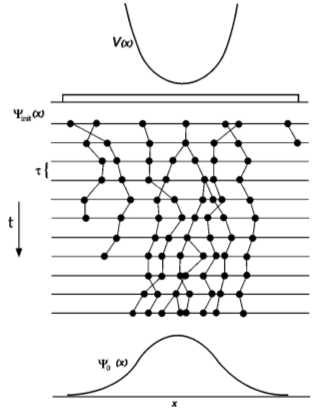
\includegraphics[width=0.9\textwidth]{branch_full.png}
\end{figure}
\end{column}
\begin{column}{0.7\textwidth}
   {\color{blue}{Figure:}} Reprinted from W.M.C. Foulkes et al. \textit{Rev. Mod. Phys.,} 73:33-83, 2001.
\end{column}
\end{columns}
\end{frame}

\begin{frame}{Diffusion Monte Carlo - Implementation}
\begin{enumerate}
   \item Start with N configurations (walkers) from VMC
   \item Loop over each walker and do the following
   \begin{enumerate}
      \setlength\itemsep{0.2em}
      \item Propose a move, $\R' = \R + \chi$, where $\chi$ is a vector of random numbers from the shifted Gaussian $\exp\left(\frac{m}{2\hbar^2\Delta\tau}\left(\R'-\R+2\frac{\nabla\Psi_I(\R')}{\Psi_I(\R')}\right)^2\right)$.
      \item The move is then accepted with the probability $A(\R'\leftarrow\R)=\mathrm{min}\left(1,\frac{\Psi_T^2(\R')}{\Psi_T^2(\R)}\right)$.
      \item Calculate the weight $w(\R')=\exp\left(-\left(E_L(\R')+E_L(\R)-2E_0\right)\Delta\tau/2\right)$.
      \item Do branching.
      \item Calculate and collect the observables and uncertainties needed and increase the imaginary time by $\Delta\tau$.
   \end{enumerate}
   \item Repeat from step 2 to 6 until the uncertainties are small enough.
\end{enumerate}
\end{frame}
\fi

\subsection{DMC}
\begin{frame}{Diffusion Monte Carlo}
\begin{itemize}
   \item DMC uses a Green's function to project out the ground state, but has no variational principle like VMC.
   \begin{equation*}
      H\Psi = i\hbar\frac{d\Psi}{dt} ~ \xrightarrow{\tau=it/\hbar} ~ H\Psi = -\frac{d\Psi}{d\tau}
   \end{equation*}
   \item The propagated wave function can be written
   \begin{equation*}
      \braket{\R'}{\Psi_T(\tau)} = \int d\R \bra{\R'}e^{-(H-E_0)\tau}\ket{\R}\braket{\R}{\Psi_T(0)}
   \end{equation*}
   \item Now we break up the propagator into small time steps $\dt = \tau/N$ and use the Trotter decomposition $e^{-H\Delta\tau}=e^{-V\Delta\tau/2}e^{-T\Delta\tau}e^{-V\Delta\tau/2}+\mathcal{O}(\Delta\tau^3)$.
   \begin{equation*}
      \braket{\R_N}{\Psi_T(\tau)} = \int d\R_1 \ldots d\R_N \left[\prod\limits_{i=1}^N G(\R_i,\R_{i-1},\Delta\tau)\right] \braket{\R_0}{\Psi_T(0)}
   \end{equation*}
   \begin{equation*}
      G(\R',\R,\Delta\tau) = \bra{\R'}e^{-(H-E_0)\Delta\tau}\ket{\R}
   \end{equation*}
\end{itemize}
\end{frame}

\begin{frame}{Diffusion Monte Carlo}
\begin{itemize}
   \item In the small $\dt$ limit this propagator can be split up with the kinetic term being used to diffuse the walkers along a random path.
   \begin{equation*}
      \bra{\R'}e^{-T\Delta \tau}\ket{\R} = \left(\frac{m}{2\pi\hbar^2\Delta\tau}\right)^{3A/2}e^{-m(\R'-\R)^2/2\hbar^2\Delta\tau}
   \end{equation*}
   \item The potential term can then be used as a weight in a branching algorithm.
   \begin{equation*}
      w(\R') = e^{-\left(V\left(\R'\right)+V\left(\R\right)-2E_0\right)\Delta\tau/2}%\bra{\R'}e^{-(V-E_0)\Delta\tau}\ket{\R}
   \end{equation*}
\end{itemize}
\end{frame}

\subsection{AFDMC}
\begin{frame}{Spin Sampling}
\begin{itemize}
   \item These expectation values also have sums over all of the $2^A$ possible spin (and isospin) states.
   \item GFMC does an explicit sum over these states and has had good success doing this up to $^{12}$C.
   \begin{equation*}
   \begin{split}
      \ket{\chi_1} &= \ket{\uparrow,\uparrow,\ldots,\uparrow} \\
      \ket{\chi_2} &= \ket{\downarrow,\uparrow,\ldots,\uparrow} \\
      \vdots & \\
      \ket{\chi_{2^A}} &= \ket{\downarrow,\downarrow,\ldots,\downarrow} \\
   \end{split}
   \end{equation*}
   \item AFDMC samples these spins and each walker has a spinor with 4 spin-isospin amplitudes for each particle, $\braket{p\uparrow}{s_i}$, $\braket{p\downarrow}{s_i}$, $\braket{n\uparrow}{s_i}$, and $\braket{n\downarrow}{s_i}$.
\end{itemize}
\end{frame}

\begin{frame}{Auxiliary Field Diffusion Monte Carlo}
\begin{itemize}
   \item AFDMC samples auxiliary fields to rotate the spins/isospins of the walkers.
   \item The spin/isospin dependent part of the potential is what is used in the spin/isospin dependent part of the propagator.
   \begin{equation*}
      G_{SD}(R'S',RS,\dt) = \bra {R'S'}e^{-V_{SD}\dt} \ket{RS}
   \end{equation*}
   \begin{equation*}
      V_{SD} = \sum\limits_{p=2}^N\sum\limits_{i<j}v_p(r_{ij})\Opij
   \end{equation*}
   \item For $v_6'$, a truncation of the phenomenological Argonne $v_{18}$ potential, the operators are $\si\cdot\sj$, $\ti\cdot\tj$, $\si\cdot\sj \ti\cdot\tj$, $S_{ij}$ and $S_{ij} \ti\cdot\tj$, where $S_{ij} = 3\si\cdot\hat{r}_{ij}\sj\cdot\hat{r}_{ij}-\si\cdot\sj$
   \red{\\ What does the rest of the potential look like?}
\end{itemize}
\end{frame}

\begin{frame}{Auxiliary Field Diffusion Monte Carlo}
\begin{itemize}
   \item We want to write these operators in terms of squared single particle operators. Matricies made of the $v_p(r_{ij})$ are defined that are symmetric and 0 if $i=j$.
   \begin{equation*}
      V_{SD} = \frac{1}{2}\sum\limits_{i\alpha j\beta} \sigma_{i\alpha}A^{\sigma}_{i\alpha j\beta}\sigma_{j\beta}
      + \frac{1}{2}\sum\limits_{i\alpha j\beta} \sigma_{i\alpha}A^{\sigma\tau}_{i\alpha j\beta}\sigma_{j\beta}\ti\cdot\tj
      + \frac{1}{2}\sum\limits_{ij} A^{\tau}_{ij}\ti\cdot\tj
   \end{equation*}
   \item We can construct these matrices and then solve for their eigenvalues and eigenvectors.
\begin{align*}
   &\sum\limits_{j\beta} A^{\sigma}_{i\alpha j\beta}\psi^{\sigma}_{nj\beta} = \lambda^{\sigma}_n\psi^{\sigma}_{ni\alpha} \\
   &\sum\limits_{j\beta} A^{\sigma\tau}_{i\alpha j\beta}\psi^{\sigma\tau}_{n j\beta} = \lambda^{\sigma\tau}_n\psi^{\sigma\tau}_{ni\alpha} \\
   &\sum\limits_{j} A^{\tau}_{ij}\psi^{\tau}_{n,j} = \lambda^{\tau}_n\psi^{\tau}_{ni}
\end{align*}
\end{itemize}
\end{frame}

\begin{frame}{Auxiliary Field Diffusion Monte Carlo}
\begin{itemize}
   \item The potential can then be written in terms of the square of new single particle operators.
   \begin{equation*}
      V_{SD} = \frac{1}{2}\sum\limits_{n=1}^{3A} \left(O_{n}^{\sigma}\right)^2 \lambda_n^{\sigma}
      + \frac{1}{2}\sum\limits_{\alpha=1}^{3}\sum\limits_{n=1}^{3A} \left(O_{n\alpha}^{\sigma\tau}\right)^2 \lambda_n^{\sigma\tau}
       + \frac{1}{2}\sum\limits_{\alpha=1}^{3}\sum\limits_{n=1}^{A} \left(O_{n\alpha}^{\tau}\right)^2 \lambda_n^{\tau}
   \end{equation*}
   \begin{equation*}
   \begin{split}
      O_{n}^{\sigma} &= \sum\limits_{j\beta} \sigma_{j\beta}\psi_{nj\beta}^{\sigma} \\
      O_{n\alpha}^{\sigma\tau} &= \sum\limits_{j\beta} \tau_{j\alpha}\sigma_{j\beta}\psi_{nj\beta}^{\sigma\tau} \\
      O_{n\alpha}^{\tau} &= \sum\limits_{j} \tau_{j\alpha}\psi_{nj}^{\tau}
   \end{split}
   \end{equation*}
\end{itemize}
\end{frame}

\begin{frame}{Auxiliary Field Diffusion Monte Carlo}
\begin{itemize}
   \item Since we have squared single particle operators in the propagator we can now rewrite the propagator in terms of the Hubbard-Stratanovich transformation.
   \begin{equation*}
      e^{-\frac{1}{2}\lambda O^2} = \frac{1}{\sqrt{2\pi}} \int dx e^{-\frac{x^2}{2} + \sqrt{-\lambda}xO}
   \end{equation*}
   \item Since we have 15A operators ($3A$ for $O_{n}^{\sigma}$, $9A$ for $O_{n\alpha}^{\sigma\tau}$, and $3A$ for $O_{n\alpha}^{\tau}$), the spin-isospin dependent part of the propagator becomes
   \begin{equation*}
      G_{SD}(R'S',RS,\dt) = \prod\limits_{n=1}^{15A}\frac{1}{\sqrt{2\pi}}\int dx_n e^{-\frac{x_n^2}{2}}e^{\sqrt{-\lambda_n\dt} x_nO_n}.
   \end{equation*}
\end{itemize}
\end{frame}

\section{Trial Wave Function}
\subsection{Spin-Dependent Correlations}
\begin{frame}{Trial Wave Function}
\begin{itemize}
   \item \textbf{Calculated often:} $\Psi_T$ controls the diffusion, branching, and random walks in addition to being used to calculate expectation values and errors.
   \item \textbf{Accurate:} $\Psi_T$ is important that the trial wave function have good overlap with the ground state energy to speed up convergence of the DMC method.
   \item It needs to be accurate and computationally inexpensive so let's talk about what it should look like.
\end{itemize}
\end{frame}

\begin{frame}{Slater Determinant}
\begin{itemize}
   \item Properties:
   \begin{itemize}
      \item Antisymmetric
      \item Cluster Decomposable \\ $\ket{A+B} = \ket{A}\ket{B}$
   \end{itemize}
   \begin{textblock*}{\textwidth}(4.5cm,-6.1cm) % {block width} (coords)
      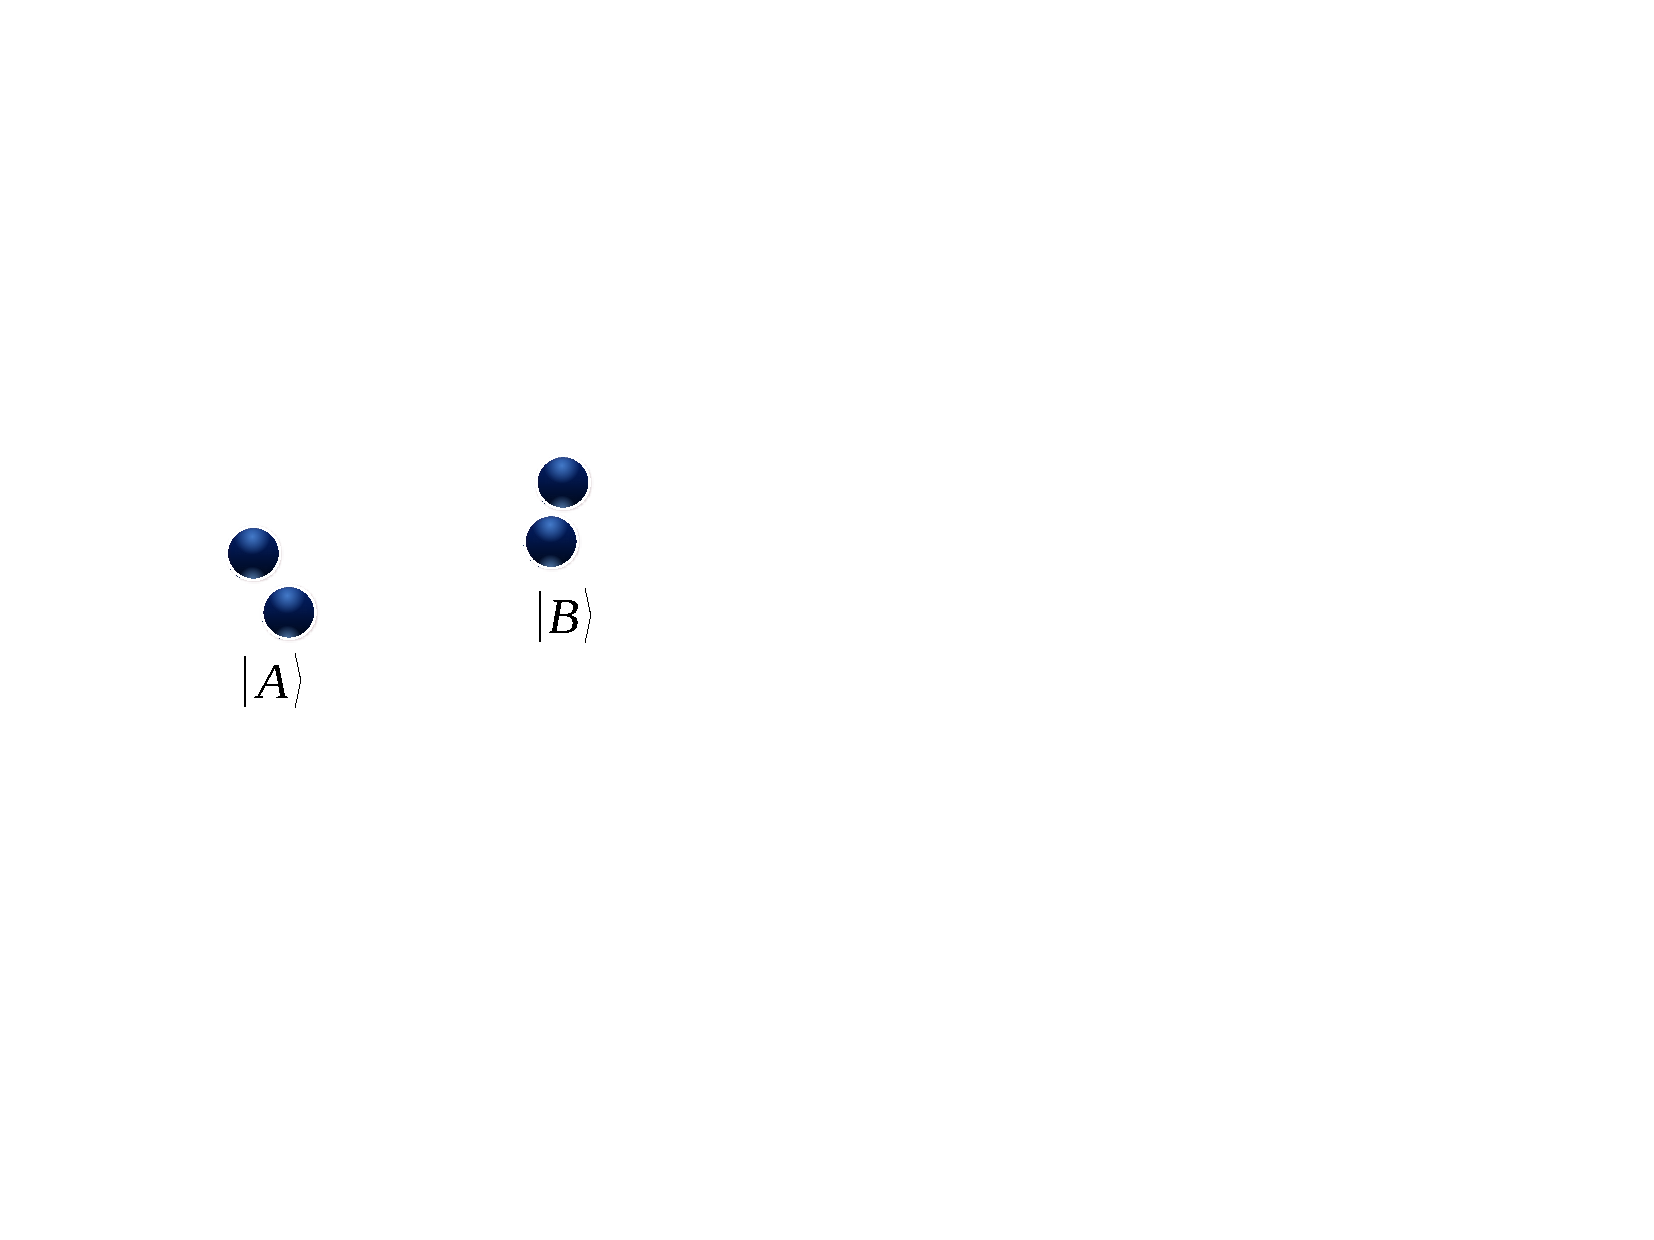
\includegraphics[width=14.6cm]{cluster.pdf}
   \end{textblock*}
   \item The simplest wave function for a many-fermion system obeying these properties is a Slater determinant where $\phi_i(\mathbf{r}_i,s_i)$ are single particle nucleon states.
   \begin{equation*}
      \psi_{T} = \braket{RS}{\phi}= \mathcal{A} \prod\limits_{i=1}^A \phi_i(\mathbf{r}_i,s_i) = \frac{1}{A!} \mathrm{det}~\phi_i(\mathbf{r}_i,s_i)
   \end{equation*}
   \item Short range correlations need to be put in by hand via Jastrow-like correlations.
   \begin{equation*}
      \ket{\psi_T} = \prod\limits_{i<j}f(r_{ij}) \ket{\phi}.
   \end{equation*}
\end{itemize}
\end{frame}

\begin{frame}{Spin Dependent Correlations}
\begin{itemize}
   \item Two spin dependent wave functions that obey these two properties are the exponentially correlated and symmetrized product wave functions.
   \begin{equation*}
      \ket{\psi_T} = \left[\prod\limits_{i<j}f_c(r_{ij})\right] e^{\sum\limits_{i<j}\sum\limits_p\fpij\Opij} \ket{\phi}
   \end{equation*}
   \begin{equation*}
      \ket{\psi_T} = \left[\prod\limits_{i<j}f_c(r_{ij})\right] \mathcal{S}\prod\limits_{i<j}\left(1+\sum\limits_p\fpij\Opij\right) \ket{\phi}
   \end{equation*}
   \item These two wave functions are the same up to second order except for  terms.
\end{itemize}
\end{frame}

\subsection{Quadratic Correlations}
\begin{frame}{Symmetrized Product Wave Function}
\begin{itemize}
   \item The symmetrized product is expensive to calculate and so an expansion truncated at linear order has been used in the past with good success.
   \begin{equation*}
      \ket{\psi_T} = \left[\prod\limits_{i<j}f_c(r_{ij})\right] \left(1+\sum\limits_p\fpij\Opij\right) \ket{\phi}
   \end{equation*}
   \item We have taken this expansion to second order.
   \begin{equation*}
   \begin{split}
      \ket{\psi_T} &= \left[\prod\limits_{i<j}f_c(r_{ij})\right] \left[1+\fOpij\right. \\
      & + \left.\frac{1}{2}\fOpij\fOqklquad + \ldots \right] \ket{\phi}
   \end{split}
   \end{equation*}
\end{itemize}
\end{frame}

\begin{frame}{Independent Pair Correlations}
\begin{itemize}
   \item Or it can be expanded to get independent pair terms
   \begin{equation*}
   \begin{split}
      \ket{\psi_T} &= \left[\prod\limits_{i<j}f_c(r_{ij})\right] \left[1+\fOpij\right. \\
      & + \left.\beta\fOpij\fOqklip + \ldots \right] \ket{\phi}
   \end{split}
   \end{equation*}
\end{itemize}
\begin{figure}[h]
   \centering
   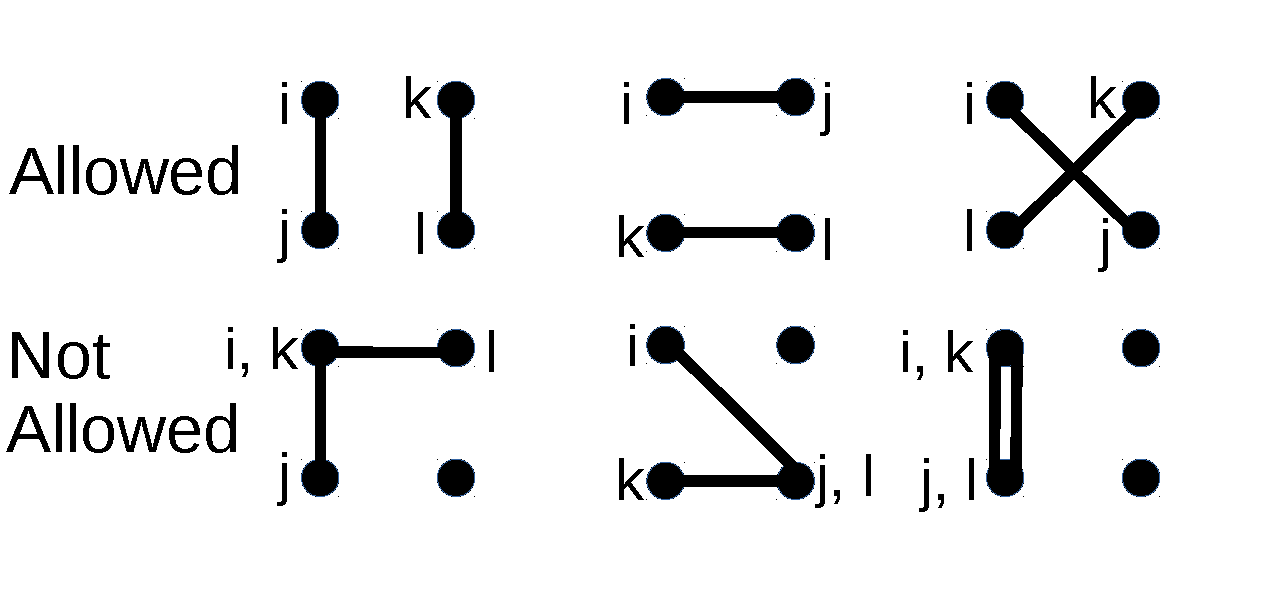
\includegraphics[width=0.7\textwidth]{pairing.pdf}
\end{figure}
\end{frame}

\begin{frame}{Results}
\begin{textblock*}{\textwidth}(0.0cm,-0.6cm) % {block width} (coords)
\begin{figure}[h]
   \centering
   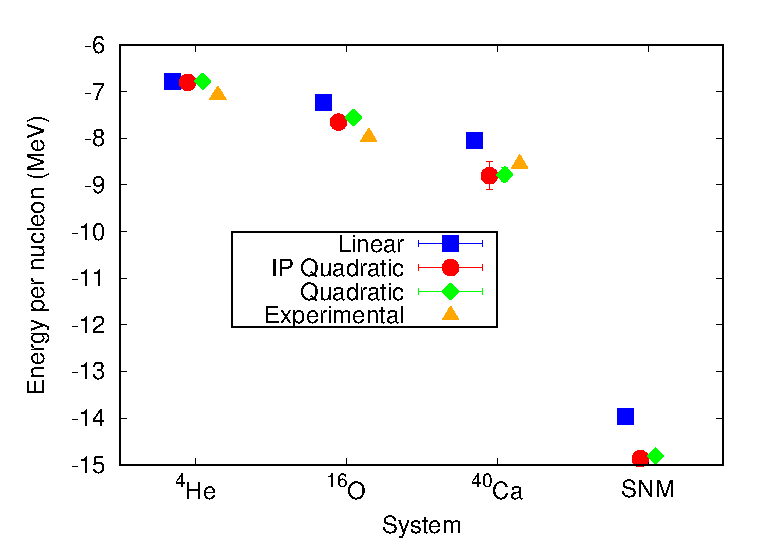
\includegraphics[width=0.6\textwidth]{energy.eps}
\end{figure}
\end{textblock*}
~\\~\\~\\~\\~\\~\\~\\~\\~\\
\tiny
\begin{table}[htb]
\centering
\caption*[]{Energy (*per nucleon) in MeV}
\begin{tabular}{ccccc}
\hline\hline
System & Linear & Ind-Pair & Quadratic & Experimental\\
\hline
${}^{4}${He}   & -27.14(4) & -27.22(3)    & -27.11(3)    & -28.295   \\
${}^{16}${O}   & -115.7(9) & -121.5(1.5)  & -120.0(1.4)  & -127.62   \\
${}^{40}${Ca}  & -324(3)   & -347(8)      & -349(5)      & -342.1     \\
SNM*           & -13.92(6) & -14.80(7)    & -14.70(11)   &           \\
\hline\hline
\end{tabular}
\label{tab:psi2}
\end{table}
{\tiny D. Lonardoni et al. \textit{Phys. Rev. C.,} \textbf{97}, 044318, 2018.}
\end{frame}

\begin{frame}{Quadratic Correlation Cost}
\begin{figure}[h]
   \centering
   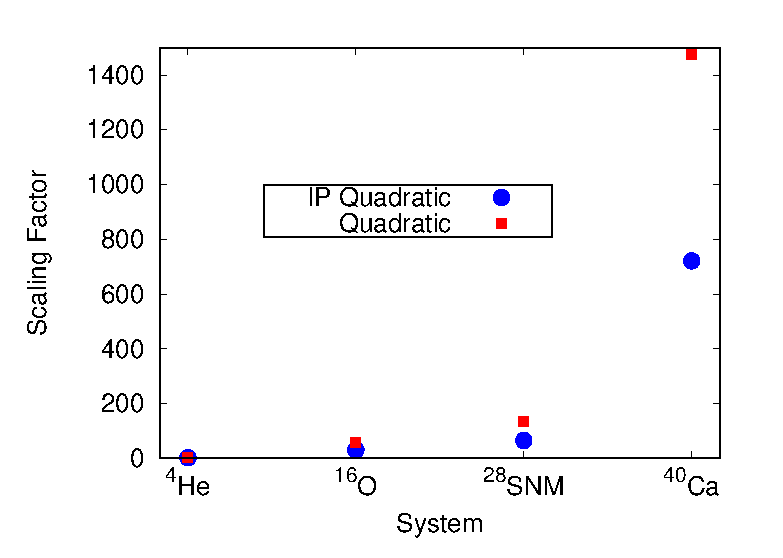
\includegraphics[width=0.65\textwidth]{scaling.eps}
\end{figure}
\begin{table}[h!]
   \centering
   \begin{tabular}{ccccc}
      \hline \hline
       & $^{4}$He & $^{16}$O & SNM(28) & $^{40}$Ca \\
      \hline
      Independent Pair & 1.73 & 30.7 & 64.8 & 720.9 \\
      Quadratic & 2.00 & 58.8 & 133.6 & 1473.9 \\
      \hline \hline
   \end{tabular}
\end{table}
\end{frame}

\subsection{Exponential Correlations}
\begin{frame}{Exponential Correlations}
\begin{itemize}
   \item The quadratic correlations improved the trial wave function, but with a large computational cost. Can we do better with the exponential correlations?
   \begin{equation*}
      \ket{\psi_T} = \left[\prod\limits_{i<j}f_c(r_{ij})\right] e^{\sum\limits_{i<j}\sum\limits_p\fpij\Opij} \ket{\phi}
   \end{equation*}
   \item We don't know how to calculate the exponential of two-body operators. But remember that we tackled this exact problem with the spin sampling in AFDMC by using the Hubbard-Stratanovich transformation.
\begin{equation*}
      e^{-\frac{1}{2}\lambda O^2} = \frac{1}{\sqrt{2\pi}} \int dx e^{-\frac{x^2}{2} + \sqrt{-\lambda}xO}
   \end{equation*}
\end{itemize}
\end{frame}

\begin{frame}{Exponential Correlations}
\begin{itemize}
   \item Following the same procedure detailed before about AFDMC spin sampling we can write the exponential correlations as
   \begin{equation*}
      \exp\left(\sum\limits_{i<j,p}f_p(r_{ij})\Oijp\right) = \exp\left(\frac{1}{2}\sum\limits_{n=1}^{15A} \left(O_{n}\right)^2 \lambda_n^{\sigma}\right),
%         &= \left[\prod\limits_{i<j}f_c(r_{ij})\right] e^{\frac{1}{2}\sum\limits_{n=1}^{3A} \left(O_{n}^{\sigma}\right)^2 \lambda_n^{\sigma}
%         + \frac{1}{2}\sum\limits_{\alpha=1}^{3}\sum\limits_{n=1}^{3A} \left(O_{n\alpha}^{\sigma\tau}\right)^2 \lambda_n^{\sigma\tau}
%         + \frac{1}{2}\sum\limits_{\alpha=1}^{3}\sum\limits_{n=1}^{A} \left(O_{n\alpha}^{\tau}\right)^2 \lambda_n^{\tau}} \ket{\phi}
   \end{equation*}
   where the $3A$ $O_{n}^{\sigma}$, $9A$ $O_{n\alpha}^{\sigma\tau}$, and $3A$ $O_{n\alpha}^{\tau}$ single particle operators are
   \begin{equation*}
   \begin{split}
      O_{n}^{\sigma} &= \sum\limits_{j,\beta} \sigma_{j,\beta}\psi_{n,j,\beta}^{\sigma} \\
      O_{n\alpha}^{\sigma\tau} &= \sum\limits_{j,\beta} \tau_{j,\alpha}\sigma_{j,\beta}\psi_{n,j,\beta}^{\sigma\tau} \\
      O_{n\alpha}^{\tau} &= \sum\limits_{j} \tau_{j,\alpha}\psi_{n,j}^{\tau}.
   \end{split}
   \end{equation*}
\end{itemize}
\end{frame}

\begin{frame}{Exponential Correlations}
\begin{itemize}
   \item Using the Hubbard-Stratanovich transformation this can then be written as
   \begin{equation}
      \exp\left(\frac{1}{2}\sum\limits_{n=1}^{15A} \left(O_{n}\right)^2 \lambda_n^{\sigma}\right) = \prod\limits_{n=1}^{15A} \frac{1}{\sqrt{2\pi}}\int dx_n e^{-x_n^2/2}e^{\sqrt{\lambda_n}x_nO_n},
   \end{equation}
   and the auxiliary fields can be sampled to be
   \begin{equation}
      \Psi_T(R,S) = \bra{RS}\prod\limits_{n=1}^{15A} \frac{1}{N} \sum\limits_{\{x_n\}}^N\frac{1}{\sqrt{2\pi}}e^{\sqrt{\lambda_n}x_nO_n}\ket{\Phi}.
   \end{equation}
\end{itemize}
\end{frame}

\begin{frame}{Exponential Correlations}
\begin{itemize}
   \item Problems with statistical errors related to the sampling. \red{Understand where these errors are coming from}.
   \item Calculating the potential energy with exponential correlations and the rest with linear correlations.
   \begin{columns}
   \begin{column}{0.5\textwidth}
   \begin{figure}[h]
      \centering
      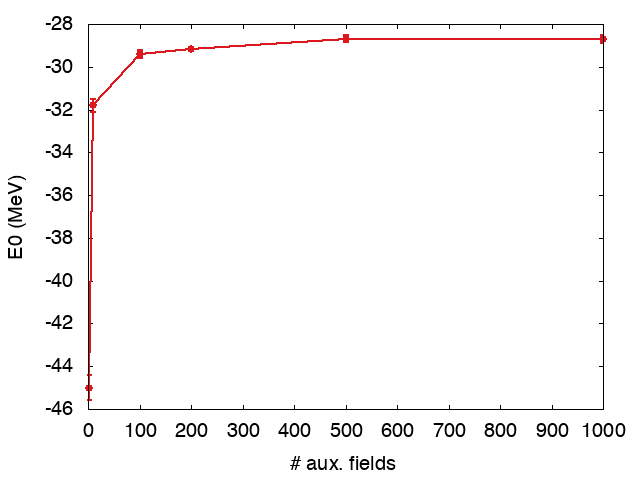
\includegraphics[width=\textwidth]{expplot.png}
   \end{figure}
   \end{column}
   \begin{column}{0.5\textwidth}
   \begin{table}[h!]
      \centering
      \caption{$^{4}$He energy with exp correlations. E$_\text{linear}$=-26.48(9) MeV.}
      \begin{tabular}{cc}
         \hline \hline
         \# fields & E (MeV) \\
         \hline
         1     & -45.0(6)  \\
         10    & -31.8(3)  \\
         100   & -29.4(2)  \\
         200   & -29.15(8) \\
         500   & -28.68(18)\\
         1000  & -28.7(2)  \\
         \hline \hline
      \end{tabular}
   \end{table}
   \end{column}
   \end{columns}
   \item Further work may be worth a look.
\end{itemize}
\end{frame}

\section{Application}
\subsection{Alpha Clustering}
\begin{frame}{Neutron Stars}
\begin{itemize}
   \item Can we use these tools to understand neutron stars?
\end{itemize}
\begin{figure}[h]
   \centering
   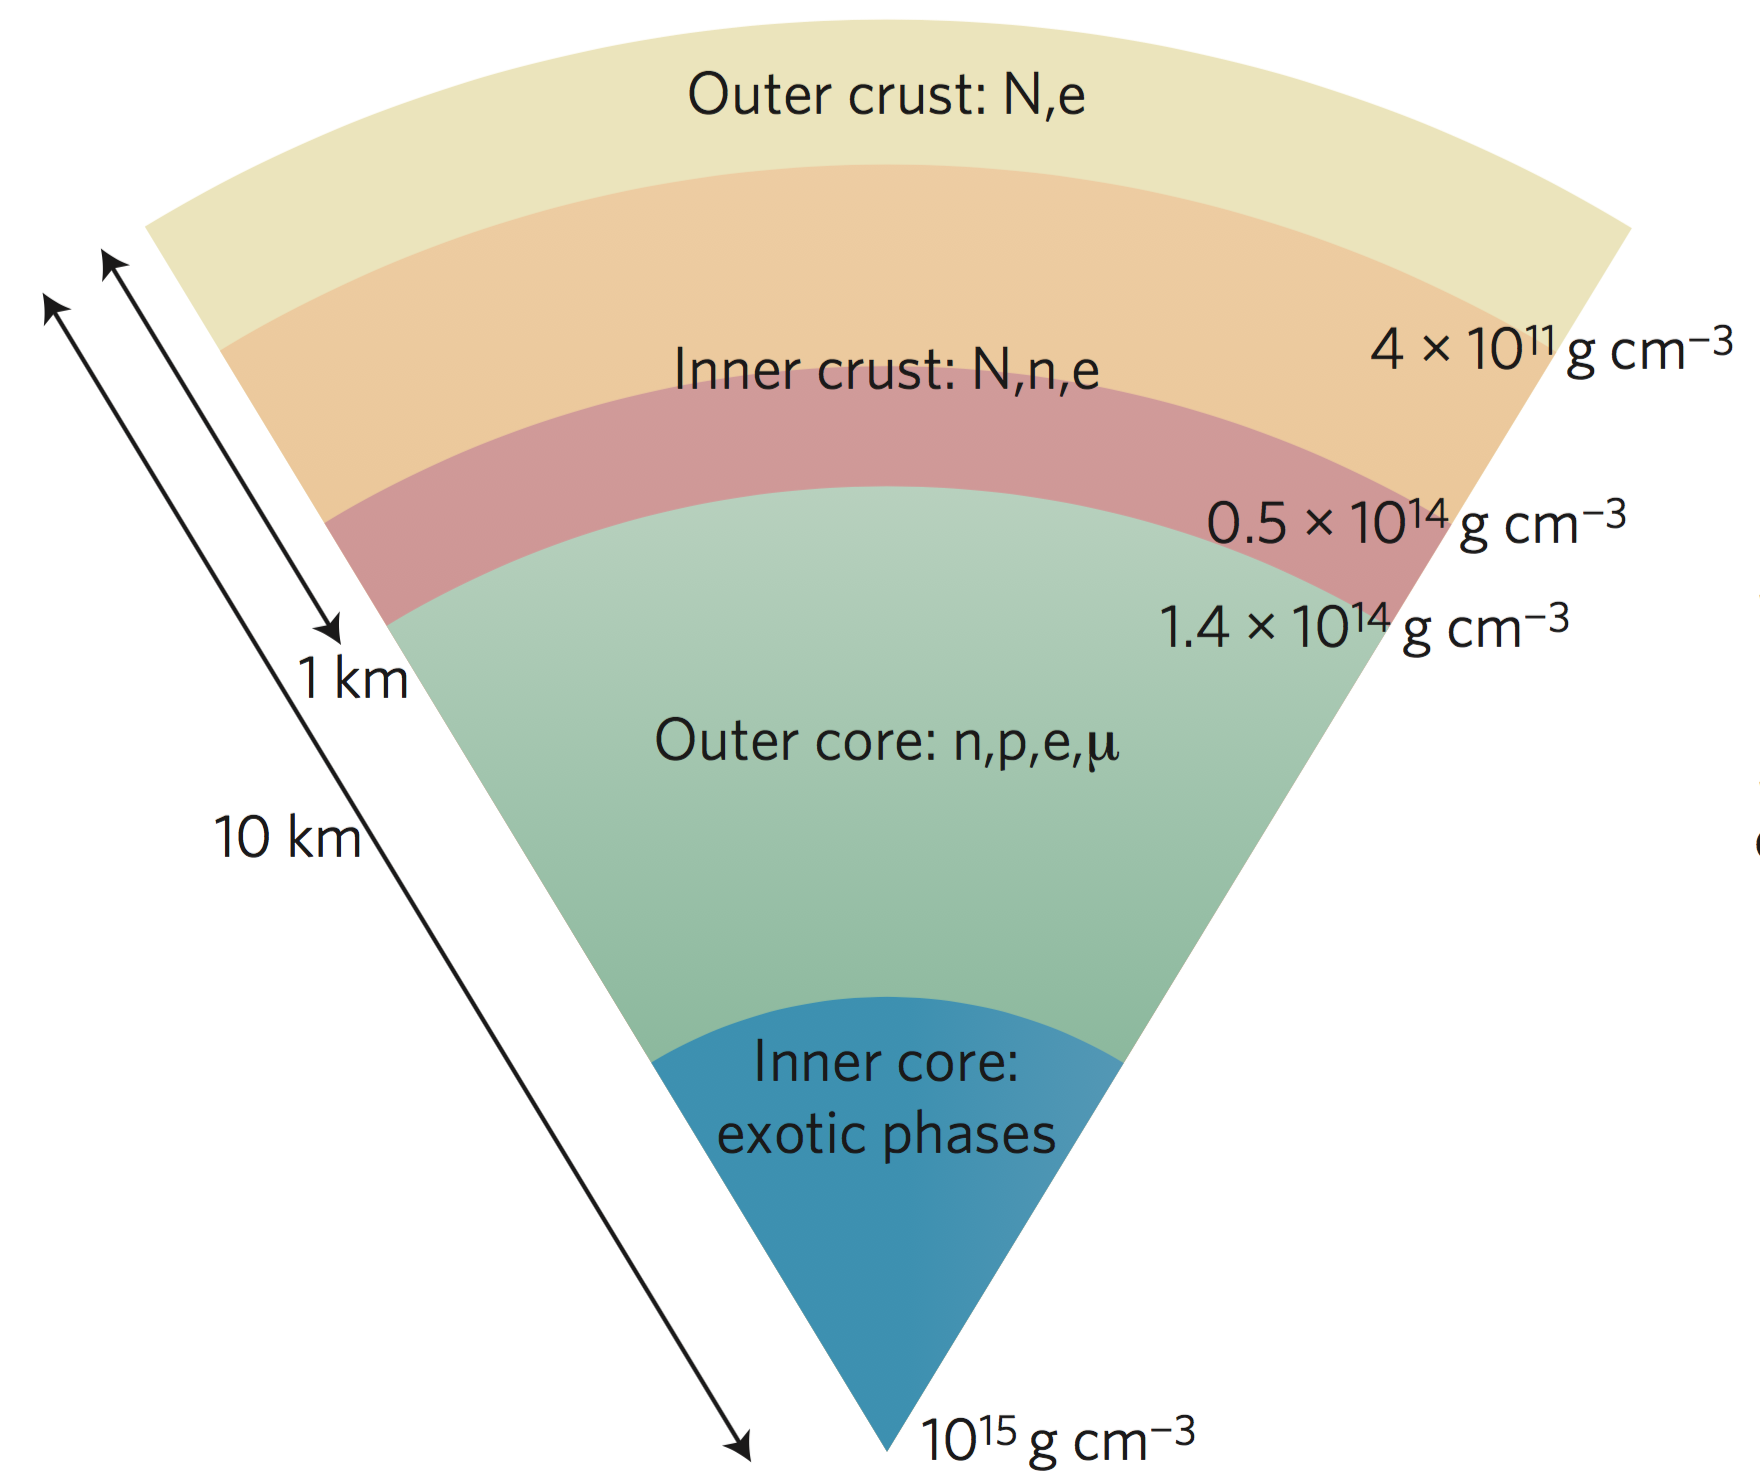
\includegraphics[width=0.5\textwidth]{neutronstar.png}
\end{figure}
W. Newton {\it Nature Physics} {\bf 9}, 396-397 (2013)
\begin{textblock*}{\textwidth}(8.1cm,-4.6cm) % {block width} (coords)
   \tiny $\approx$ 0.00024 fm$^{-3}$
\end{textblock*}
\begin{textblock*}{\textwidth}(7.8cm,-4.1cm) % {block width} (coords)
   \tiny $\approx$ 0.030 fm$^{-3}$
\end{textblock*}
\begin{textblock*}{\textwidth}(7.6cm,-3.8cm) % {block width} (coords)
   \tiny $\approx$ 0.084 fm$^{-3}$
\end{textblock*}
\begin{textblock*}{\textwidth}(6.4cm,-1.3cm) % {block width} (coords)
   \tiny $\approx$ 0.60 fm$^{-3}$
\end{textblock*}
\end{frame}

\begin{frame}{Alpha Particle Clustering in Mostly Neutron Matter}
\begin{itemize}
   \item If alpha particles form in nearly neutron matter then we should be able to estimate their energy by
   \begin{equation*}
      E_\alpha = E_\text{14n+2p} - E_\text{12n}
   \end{equation*}
   \begin{columns}
   \begin{column}{0.5\textwidth}
   \begin{figure}[h]
      \centering
      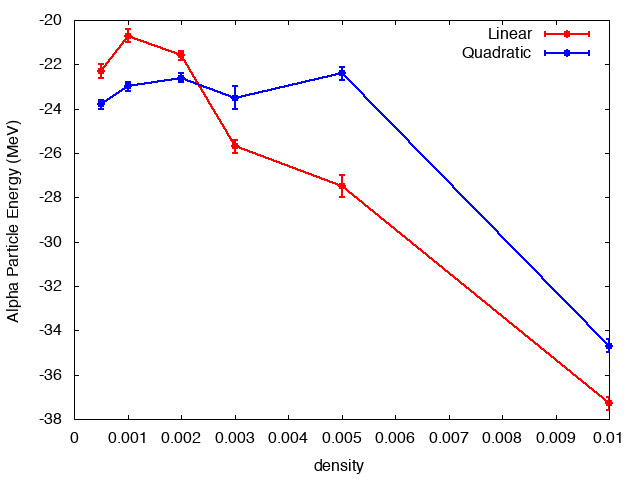
\includegraphics[width=\textwidth]{clusterplot.png}
   \end{figure}
   \end{column}
   \begin{column}{0.5\textwidth}
   \begin{table}[h!]
      \centering
      \caption{Alpha energy in MeV}
      \begin{tabular}{ccc}
         \hline \hline
         $\rho$ (fm$^{-3}$) & lin & ip \\
         \hline
         0.0005& -22.3(3)  & -23.8(2)  \\
         0.001 & -20.7(3)  & -23.0(2)  \\
         0.002 & -21.6(2)  & -22.6(2)  \\
         0.003 & -25.7(3)  & -23.5(5)  \\
         0.005 & -27.5(5)  & -22.4(3)  \\
         0.01  & -37.3(3)  & -34.7(3)  \\
         \hline \hline
      \end{tabular}
   \end{table}
   \end{column}
   \end{columns}
\end{itemize}
\end{frame}

%\note[itemize]{
%   \item test1
%   \item test2
%}

\begin{frame}{Extra Slides}
Extra Slides
\end{frame}

\begin{frame}{Diffusion Monte Carlo - Branching}
Branching: Each walker can be deleted or multiply. The number of walkers that continues is equal to $\mathrm{int}\left(w(\R')+\xi\right)$, where $\xi$ is a uniform random number from $[0,1]$.
\begin{columns}
\begin{column}{0.4\textwidth}
\begin{figure}
   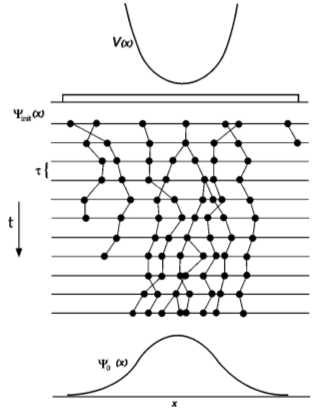
\includegraphics[width=0.9\textwidth]{branch_full.png}
\end{figure}
\end{column}
\begin{column}{0.7\textwidth}
   {\color{blue}{Figure:}} Reprinted from W.M.C. Foulkes et al. \textit{Rev. Mod. Phys.,} 73:33-83, 2001.
\end{column}
\end{columns}
\end{frame}

\end{document}
